\begin{frame}[t,fragile]{計算グラフ}
  \begin{itemize}
    %\setlength{\itemsep}{1em}
  \item 任意の関数の計算過程は、入力値と基本演算からなる計算グラフ(computation graph)で表現できる

    例: $\displaystyle f(x_1,x_2,x_3) = \frac{(x_1 - \exp(x_2)) x_3 \exp(x_2)}{x_3 \exp(x_2) + 1}$
    \begin{center}
      \resizebox{.45\textwidth}{!}{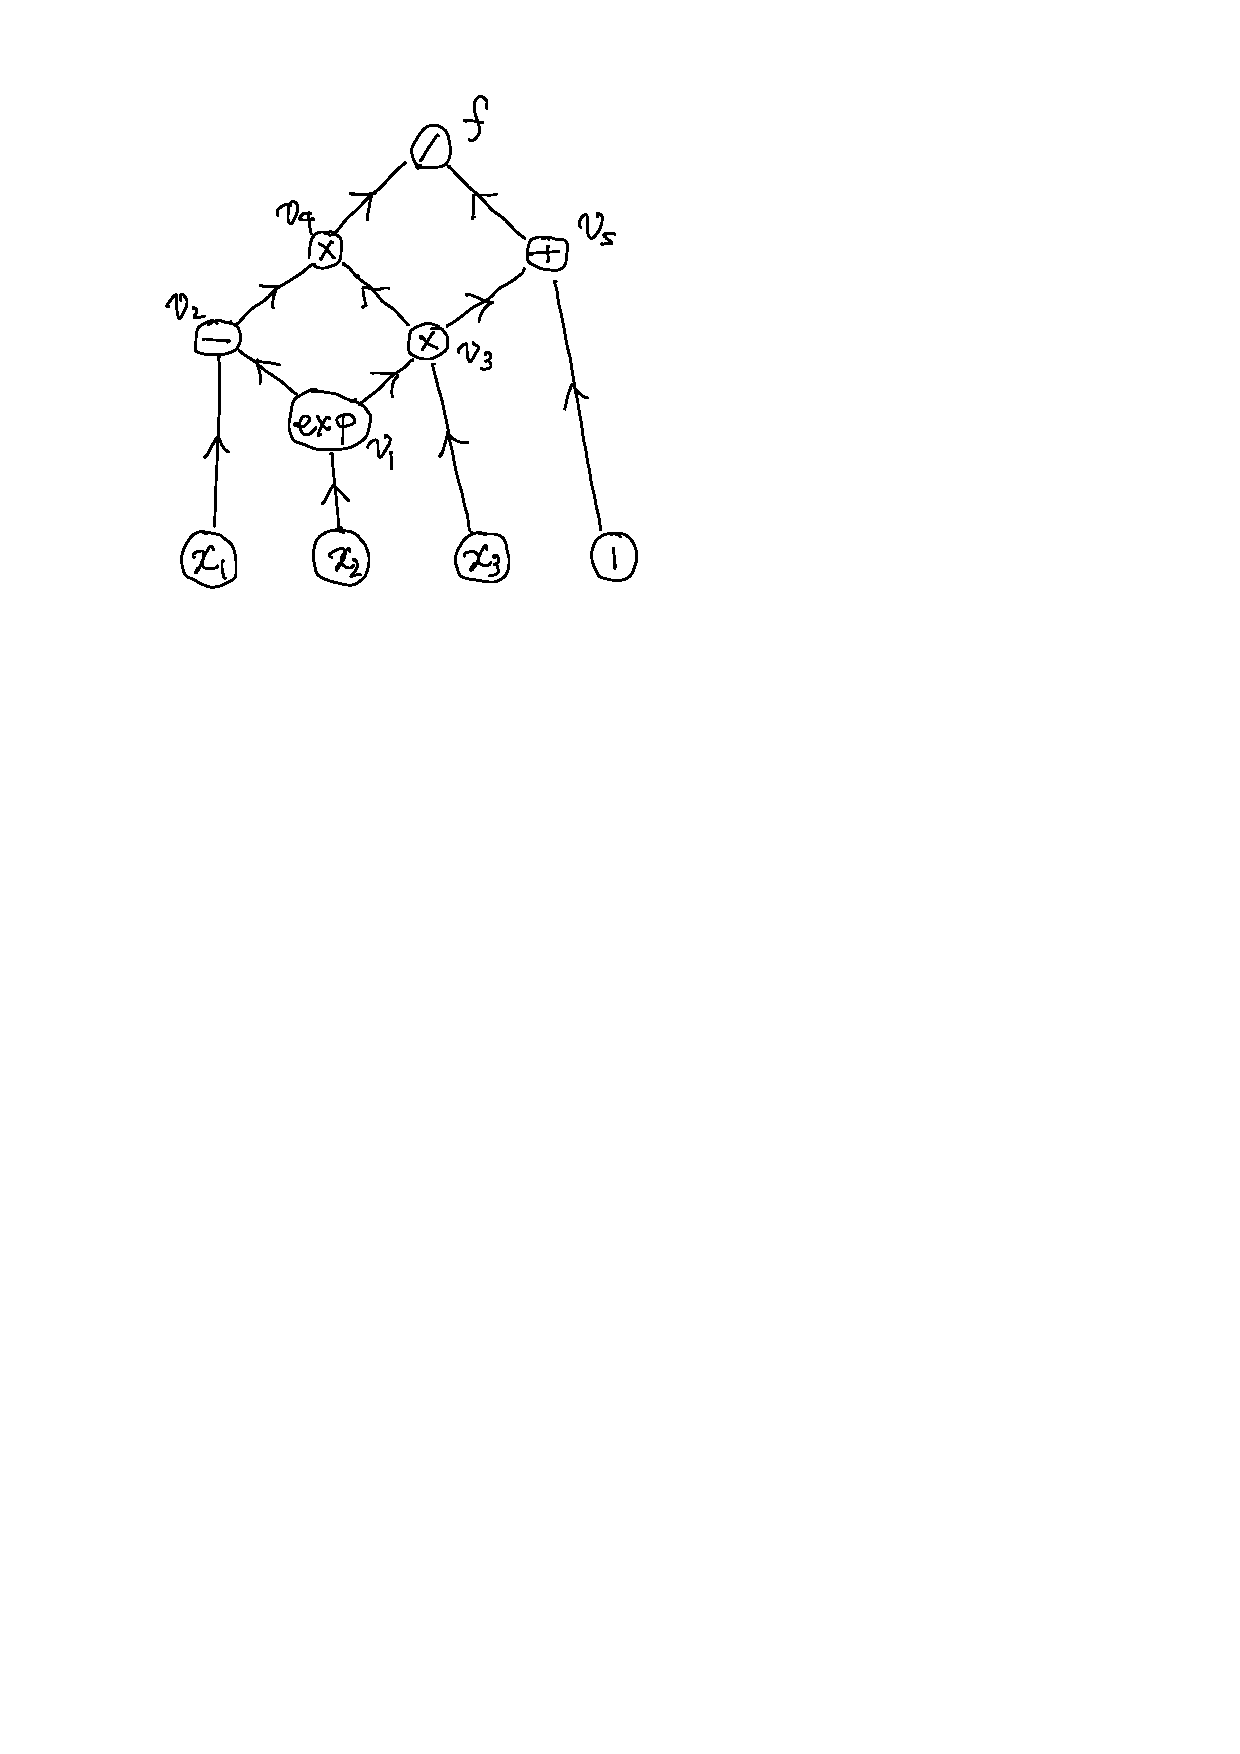
\includegraphics{image/compgraph.pdf}}
    \end{center}
    \vspace*{-2em} \hfill {\footnotesize [伊理・久保田(1991)]}
  \end{itemize}
\end{frame}
